\subsection{Exploratory Search}
(Ilkka)

\begin{figure*}[htp] % t=top, h=here, b=bottom, p=separate page, !=place even if ugly
\caption{Different search tasks are split into three overlapping search activities: \textit{lookup}, \textit{learn} and \textit{investigate}. Based on \protect\cite{march06}.}
\label{figure_3clouds}
\centering
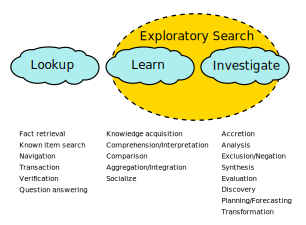
\includegraphics[scale=1.5]{figures/3clouds.pdf}
\end{figure*}

Introduction to exploratory search. See Figure \ref{figure_3clouds}.
\cite{march06}, \cite{white09}, \cite{tvaro11}

The user interface of an exploratory search system should be designed to fulfill the needs of most of its users. More information on what works and doesn't work can usually be collected from system evaluations.

However, evaluating exploratory search systems is difficult, because users have different starting positions. Their knowledge of the domain varies, they are interested in different aspects of the topic and they have previously encountered different information. \cite{kules08}

Exploratory search and iterative search differ. See Figure \ref{figure_IterativeVsExploratory}.

\begin{figure}[htp] % t=top, h=here, b=bottom, p=separate page, !=place even if ugly
\caption{They differ. Based on \protect\cite{white09}.}
\label{figure_IterativeVsExploratory}
\centering
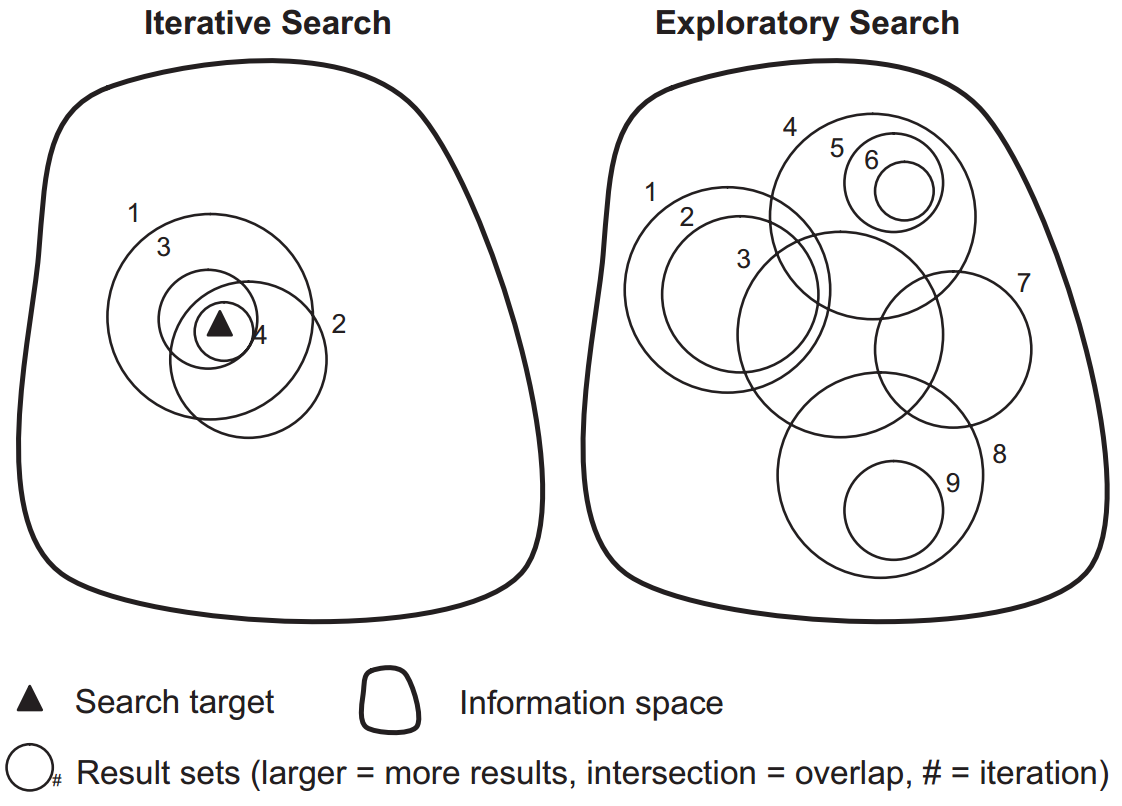
\includegraphics[scale=0.2]{figures/IterativeSearch_vs_ExploratorySearch.pdf}
\end{figure}

Exploratory search tasks can be characterized as either learning oriented or investigative  and they have common aspects like uncertainty, ambiguity and discovery distinguishing them from look-up oriented tasks \cite{kules09}.

